% Created by tikzDevice version 0.12
% !TEX encoding = UTF-8 Unicode
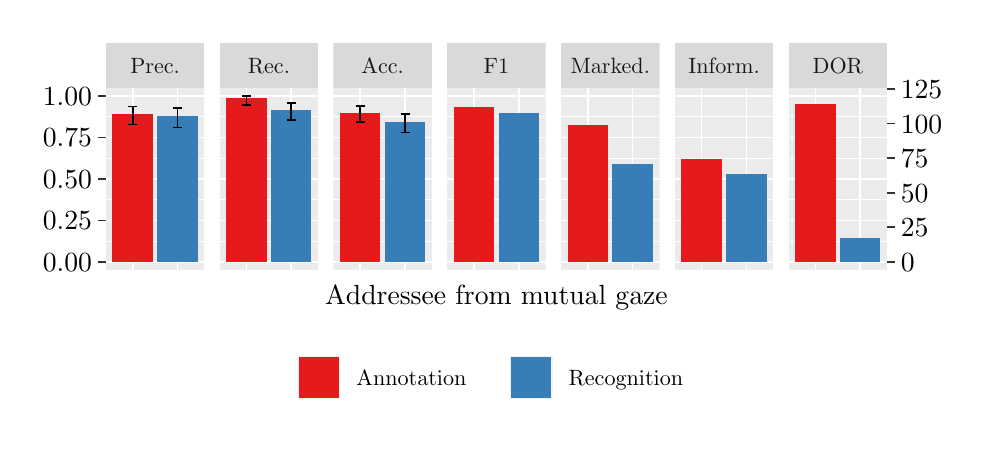
\begin{tikzpicture}[x=1pt,y=1pt]
\definecolor{fillColor}{RGB}{255,255,255}
\path[use as bounding box,fill=fillColor,fill opacity=0.00] (0,0) rectangle (336.00,145.35);
\begin{scope}
\path[clip] (  0.00,  0.00) rectangle (336.00,145.35);
\definecolor{drawColor}{RGB}{255,255,255}
\definecolor{fillColor}{RGB}{255,255,255}

\path[draw=drawColor,line width= 0.6pt,line join=round,line cap=round,fill=fillColor] (  0.00,  0.00) rectangle (336.00,145.35);
\end{scope}
\begin{scope}
\path[clip] ( 28.22, 57.73) rectangle ( 63.84,123.60);
\definecolor{fillColor}{gray}{0.92}

\path[fill=fillColor] ( 28.22, 57.73) rectangle ( 63.84,123.60);
\definecolor{drawColor}{RGB}{255,255,255}

\path[draw=drawColor,line width= 0.3pt,line join=round] ( 28.22, 68.22) --
	( 63.84, 68.22);

\path[draw=drawColor,line width= 0.3pt,line join=round] ( 28.22, 83.22) --
	( 63.84, 83.22);

\path[draw=drawColor,line width= 0.3pt,line join=round] ( 28.22, 98.22) --
	( 63.84, 98.22);

\path[draw=drawColor,line width= 0.3pt,line join=round] ( 28.22,113.22) --
	( 63.84,113.22);

\path[draw=drawColor,line width= 0.6pt,line join=round] ( 28.22, 60.72) --
	( 63.84, 60.72);

\path[draw=drawColor,line width= 0.6pt,line join=round] ( 28.22, 75.72) --
	( 63.84, 75.72);

\path[draw=drawColor,line width= 0.6pt,line join=round] ( 28.22, 90.72) --
	( 63.84, 90.72);

\path[draw=drawColor,line width= 0.6pt,line join=round] ( 28.22,105.72) --
	( 63.84,105.72);

\path[draw=drawColor,line width= 0.6pt,line join=round] ( 28.22,120.72) --
	( 63.84,120.72);

\path[draw=drawColor,line width= 0.6pt,line join=round] ( 37.94, 57.73) --
	( 37.94,123.60);

\path[draw=drawColor,line width= 0.6pt,line join=round] ( 54.13, 57.73) --
	( 54.13,123.60);
\definecolor{fillColor}{RGB}{228,26,28}

\path[fill=fillColor] ( 30.65, 60.72) rectangle ( 45.22,114.14);
\definecolor{fillColor}{RGB}{55,126,184}

\path[fill=fillColor] ( 46.84, 60.72) rectangle ( 61.41,113.33);
\definecolor{drawColor}{RGB}{0,0,0}

\path[draw=drawColor,line width= 0.6pt,line join=round] ( 52.51,116.31) --
	( 55.75,116.31);

\path[draw=drawColor,line width= 0.6pt,line join=round] ( 54.13,116.31) --
	( 54.13,109.32);

\path[draw=drawColor,line width= 0.6pt,line join=round] ( 52.51,109.32) --
	( 55.75,109.32);

\path[draw=drawColor,line width= 0.6pt,line join=round] ( 36.32,116.88) --
	( 39.56,116.88);

\path[draw=drawColor,line width= 0.6pt,line join=round] ( 37.94,116.88) --
	( 37.94,110.41);

\path[draw=drawColor,line width= 0.6pt,line join=round] ( 36.32,110.41) --
	( 39.56,110.41);
\end{scope}
\begin{scope}
\path[clip] ( 69.34, 57.73) rectangle (104.96,123.60);
\definecolor{fillColor}{gray}{0.92}

\path[fill=fillColor] ( 69.34, 57.73) rectangle (104.96,123.60);
\definecolor{drawColor}{RGB}{255,255,255}

\path[draw=drawColor,line width= 0.3pt,line join=round] ( 69.34, 68.22) --
	(104.96, 68.22);

\path[draw=drawColor,line width= 0.3pt,line join=round] ( 69.34, 83.22) --
	(104.96, 83.22);

\path[draw=drawColor,line width= 0.3pt,line join=round] ( 69.34, 98.22) --
	(104.96, 98.22);

\path[draw=drawColor,line width= 0.3pt,line join=round] ( 69.34,113.22) --
	(104.96,113.22);

\path[draw=drawColor,line width= 0.6pt,line join=round] ( 69.34, 60.72) --
	(104.96, 60.72);

\path[draw=drawColor,line width= 0.6pt,line join=round] ( 69.34, 75.72) --
	(104.96, 75.72);

\path[draw=drawColor,line width= 0.6pt,line join=round] ( 69.34, 90.72) --
	(104.96, 90.72);

\path[draw=drawColor,line width= 0.6pt,line join=round] ( 69.34,105.72) --
	(104.96,105.72);

\path[draw=drawColor,line width= 0.6pt,line join=round] ( 69.34,120.72) --
	(104.96,120.72);

\path[draw=drawColor,line width= 0.6pt,line join=round] ( 79.06, 57.73) --
	( 79.06,123.60);

\path[draw=drawColor,line width= 0.6pt,line join=round] ( 95.25, 57.73) --
	( 95.25,123.60);
\definecolor{fillColor}{RGB}{228,26,28}

\path[fill=fillColor] ( 71.77, 60.72) rectangle ( 86.34,119.81);
\definecolor{fillColor}{RGB}{55,126,184}

\path[fill=fillColor] ( 87.96, 60.72) rectangle (102.53,115.72);
\definecolor{drawColor}{RGB}{0,0,0}

\path[draw=drawColor,line width= 0.6pt,line join=round] ( 93.63,118.18) --
	( 96.87,118.18);

\path[draw=drawColor,line width= 0.6pt,line join=round] ( 95.25,118.18) --
	( 95.25,112.06);

\path[draw=drawColor,line width= 0.6pt,line join=round] ( 93.63,112.06) --
	( 96.87,112.06);

\path[draw=drawColor,line width= 0.6pt,line join=round] ( 77.44,120.61) --
	( 80.68,120.61);

\path[draw=drawColor,line width= 0.6pt,line join=round] ( 79.06,120.61) --
	( 79.06,117.50);

\path[draw=drawColor,line width= 0.6pt,line join=round] ( 77.44,117.50) --
	( 80.68,117.50);
\end{scope}
\begin{scope}
\path[clip] (110.46, 57.73) rectangle (146.08,123.60);
\definecolor{fillColor}{gray}{0.92}

\path[fill=fillColor] (110.46, 57.73) rectangle (146.08,123.60);
\definecolor{drawColor}{RGB}{255,255,255}

\path[draw=drawColor,line width= 0.3pt,line join=round] (110.46, 68.22) --
	(146.08, 68.22);

\path[draw=drawColor,line width= 0.3pt,line join=round] (110.46, 83.22) --
	(146.08, 83.22);

\path[draw=drawColor,line width= 0.3pt,line join=round] (110.46, 98.22) --
	(146.08, 98.22);

\path[draw=drawColor,line width= 0.3pt,line join=round] (110.46,113.22) --
	(146.08,113.22);

\path[draw=drawColor,line width= 0.6pt,line join=round] (110.46, 60.72) --
	(146.08, 60.72);

\path[draw=drawColor,line width= 0.6pt,line join=round] (110.46, 75.72) --
	(146.08, 75.72);

\path[draw=drawColor,line width= 0.6pt,line join=round] (110.46, 90.72) --
	(146.08, 90.72);

\path[draw=drawColor,line width= 0.6pt,line join=round] (110.46,105.72) --
	(146.08,105.72);

\path[draw=drawColor,line width= 0.6pt,line join=round] (110.46,120.72) --
	(146.08,120.72);

\path[draw=drawColor,line width= 0.6pt,line join=round] (120.17, 57.73) --
	(120.17,123.60);

\path[draw=drawColor,line width= 0.6pt,line join=round] (136.37, 57.73) --
	(136.37,123.60);
\definecolor{fillColor}{RGB}{228,26,28}

\path[fill=fillColor] (112.89, 60.72) rectangle (127.46,114.58);
\definecolor{fillColor}{RGB}{55,126,184}

\path[fill=fillColor] (129.08, 60.72) rectangle (143.65,111.17);
\definecolor{drawColor}{RGB}{0,0,0}

\path[draw=drawColor,line width= 0.6pt,line join=round] (134.75,114.21) --
	(137.98,114.21);

\path[draw=drawColor,line width= 0.6pt,line join=round] (136.37,114.21) --
	(136.37,107.42);

\path[draw=drawColor,line width= 0.6pt,line join=round] (134.75,107.42) --
	(137.98,107.42);

\path[draw=drawColor,line width= 0.6pt,line join=round] (118.56,117.01) --
	(121.79,117.01);

\path[draw=drawColor,line width= 0.6pt,line join=round] (120.17,117.01) --
	(120.17,111.31);

\path[draw=drawColor,line width= 0.6pt,line join=round] (118.56,111.31) --
	(121.79,111.31);
\end{scope}
\begin{scope}
\path[clip] (151.58, 57.73) rectangle (187.20,123.60);
\definecolor{fillColor}{gray}{0.92}

\path[fill=fillColor] (151.58, 57.73) rectangle (187.20,123.60);
\definecolor{drawColor}{RGB}{255,255,255}

\path[draw=drawColor,line width= 0.3pt,line join=round] (151.58, 68.22) --
	(187.20, 68.22);

\path[draw=drawColor,line width= 0.3pt,line join=round] (151.58, 83.22) --
	(187.20, 83.22);

\path[draw=drawColor,line width= 0.3pt,line join=round] (151.58, 98.22) --
	(187.20, 98.22);

\path[draw=drawColor,line width= 0.3pt,line join=round] (151.58,113.22) --
	(187.20,113.22);

\path[draw=drawColor,line width= 0.6pt,line join=round] (151.58, 60.72) --
	(187.20, 60.72);

\path[draw=drawColor,line width= 0.6pt,line join=round] (151.58, 75.72) --
	(187.20, 75.72);

\path[draw=drawColor,line width= 0.6pt,line join=round] (151.58, 90.72) --
	(187.20, 90.72);

\path[draw=drawColor,line width= 0.6pt,line join=round] (151.58,105.72) --
	(187.20,105.72);

\path[draw=drawColor,line width= 0.6pt,line join=round] (151.58,120.72) --
	(187.20,120.72);

\path[draw=drawColor,line width= 0.6pt,line join=round] (161.29, 57.73) --
	(161.29,123.60);

\path[draw=drawColor,line width= 0.6pt,line join=round] (177.48, 57.73) --
	(177.48,123.60);
\definecolor{fillColor}{RGB}{228,26,28}

\path[fill=fillColor] (154.01, 60.72) rectangle (168.58,116.83);
\definecolor{fillColor}{RGB}{55,126,184}

\path[fill=fillColor] (170.20, 60.72) rectangle (184.77,114.49);
\end{scope}
\begin{scope}
\path[clip] (192.70, 57.73) rectangle (228.32,123.60);
\definecolor{fillColor}{gray}{0.92}

\path[fill=fillColor] (192.70, 57.73) rectangle (228.32,123.60);
\definecolor{drawColor}{RGB}{255,255,255}

\path[draw=drawColor,line width= 0.3pt,line join=round] (192.70, 68.22) --
	(228.32, 68.22);

\path[draw=drawColor,line width= 0.3pt,line join=round] (192.70, 83.22) --
	(228.32, 83.22);

\path[draw=drawColor,line width= 0.3pt,line join=round] (192.70, 98.22) --
	(228.32, 98.22);

\path[draw=drawColor,line width= 0.3pt,line join=round] (192.70,113.22) --
	(228.32,113.22);

\path[draw=drawColor,line width= 0.6pt,line join=round] (192.70, 60.72) --
	(228.32, 60.72);

\path[draw=drawColor,line width= 0.6pt,line join=round] (192.70, 75.72) --
	(228.32, 75.72);

\path[draw=drawColor,line width= 0.6pt,line join=round] (192.70, 90.72) --
	(228.32, 90.72);

\path[draw=drawColor,line width= 0.6pt,line join=round] (192.70,105.72) --
	(228.32,105.72);

\path[draw=drawColor,line width= 0.6pt,line join=round] (192.70,120.72) --
	(228.32,120.72);

\path[draw=drawColor,line width= 0.6pt,line join=round] (202.41, 57.73) --
	(202.41,123.60);

\path[draw=drawColor,line width= 0.6pt,line join=round] (218.60, 57.73) --
	(218.60,123.60);
\definecolor{fillColor}{RGB}{228,26,28}

\path[fill=fillColor] (195.13, 60.72) rectangle (209.70,110.14);
\definecolor{fillColor}{RGB}{55,126,184}

\path[fill=fillColor] (211.32, 60.72) rectangle (225.89, 95.96);
\end{scope}
\begin{scope}
\path[clip] (233.82, 57.73) rectangle (269.44,123.60);
\definecolor{fillColor}{gray}{0.92}

\path[fill=fillColor] (233.82, 57.73) rectangle (269.44,123.60);
\definecolor{drawColor}{RGB}{255,255,255}

\path[draw=drawColor,line width= 0.3pt,line join=round] (233.82, 68.22) --
	(269.44, 68.22);

\path[draw=drawColor,line width= 0.3pt,line join=round] (233.82, 83.22) --
	(269.44, 83.22);

\path[draw=drawColor,line width= 0.3pt,line join=round] (233.82, 98.22) --
	(269.44, 98.22);

\path[draw=drawColor,line width= 0.3pt,line join=round] (233.82,113.22) --
	(269.44,113.22);

\path[draw=drawColor,line width= 0.6pt,line join=round] (233.82, 60.72) --
	(269.44, 60.72);

\path[draw=drawColor,line width= 0.6pt,line join=round] (233.82, 75.72) --
	(269.44, 75.72);

\path[draw=drawColor,line width= 0.6pt,line join=round] (233.82, 90.72) --
	(269.44, 90.72);

\path[draw=drawColor,line width= 0.6pt,line join=round] (233.82,105.72) --
	(269.44,105.72);

\path[draw=drawColor,line width= 0.6pt,line join=round] (233.82,120.72) --
	(269.44,120.72);

\path[draw=drawColor,line width= 0.6pt,line join=round] (243.53, 57.73) --
	(243.53,123.60);

\path[draw=drawColor,line width= 0.6pt,line join=round] (259.72, 57.73) --
	(259.72,123.60);
\definecolor{fillColor}{RGB}{228,26,28}

\path[fill=fillColor] (236.24, 60.72) rectangle (250.82, 97.99);
\definecolor{fillColor}{RGB}{55,126,184}

\path[fill=fillColor] (252.44, 60.72) rectangle (267.01, 92.54);
\end{scope}
\begin{scope}
\path[clip] (274.94, 57.73) rectangle (310.55,123.60);
\definecolor{fillColor}{gray}{0.92}

\path[fill=fillColor] (274.94, 57.73) rectangle (310.55,123.60);
\definecolor{drawColor}{RGB}{255,255,255}

\path[draw=drawColor,line width= 0.3pt,line join=round] (274.94, 68.22) --
	(310.55, 68.22);

\path[draw=drawColor,line width= 0.3pt,line join=round] (274.94, 83.22) --
	(310.55, 83.22);

\path[draw=drawColor,line width= 0.3pt,line join=round] (274.94, 98.22) --
	(310.55, 98.22);

\path[draw=drawColor,line width= 0.3pt,line join=round] (274.94,113.22) --
	(310.55,113.22);

\path[draw=drawColor,line width= 0.6pt,line join=round] (274.94, 60.72) --
	(310.55, 60.72);

\path[draw=drawColor,line width= 0.6pt,line join=round] (274.94, 75.72) --
	(310.55, 75.72);

\path[draw=drawColor,line width= 0.6pt,line join=round] (274.94, 90.72) --
	(310.55, 90.72);

\path[draw=drawColor,line width= 0.6pt,line join=round] (274.94,105.72) --
	(310.55,105.72);

\path[draw=drawColor,line width= 0.6pt,line join=round] (274.94,120.72) --
	(310.55,120.72);

\path[draw=drawColor,line width= 0.6pt,line join=round] (284.65, 57.73) --
	(284.65,123.60);

\path[draw=drawColor,line width= 0.6pt,line join=round] (300.84, 57.73) --
	(300.84,123.60);
\definecolor{fillColor}{RGB}{228,26,28}

\path[fill=fillColor] (277.36, 60.72) rectangle (291.93,117.59);
\definecolor{fillColor}{RGB}{55,126,184}

\path[fill=fillColor] (293.55, 60.72) rectangle (308.13, 69.46);
\end{scope}
\begin{scope}
\path[clip] ( 28.22,123.60) rectangle ( 63.84,139.85);
\definecolor{fillColor}{gray}{0.85}

\path[fill=fillColor] ( 28.22,123.60) rectangle ( 63.84,139.85);
\definecolor{drawColor}{gray}{0.10}

\node[text=drawColor,anchor=base,inner sep=0pt, outer sep=0pt, scale=  0.80] at ( 46.03,128.97) {Prec.};
\end{scope}
\begin{scope}
\path[clip] ( 69.34,123.60) rectangle (104.96,139.85);
\definecolor{fillColor}{gray}{0.85}

\path[fill=fillColor] ( 69.34,123.60) rectangle (104.96,139.85);
\definecolor{drawColor}{gray}{0.10}

\node[text=drawColor,anchor=base,inner sep=0pt, outer sep=0pt, scale=  0.80] at ( 87.15,128.97) {Rec.};
\end{scope}
\begin{scope}
\path[clip] (110.46,123.60) rectangle (146.08,139.85);
\definecolor{fillColor}{gray}{0.85}

\path[fill=fillColor] (110.46,123.60) rectangle (146.08,139.85);
\definecolor{drawColor}{gray}{0.10}

\node[text=drawColor,anchor=base,inner sep=0pt, outer sep=0pt, scale=  0.80] at (128.27,128.97) {Acc.};
\end{scope}
\begin{scope}
\path[clip] (151.58,123.60) rectangle (187.20,139.85);
\definecolor{fillColor}{gray}{0.85}

\path[fill=fillColor] (151.58,123.60) rectangle (187.20,139.85);
\definecolor{drawColor}{gray}{0.10}

\node[text=drawColor,anchor=base,inner sep=0pt, outer sep=0pt, scale=  0.80] at (169.39,128.97) {F1};
\end{scope}
\begin{scope}
\path[clip] (192.70,123.60) rectangle (228.32,139.85);
\definecolor{fillColor}{gray}{0.85}

\path[fill=fillColor] (192.70,123.60) rectangle (228.32,139.85);
\definecolor{drawColor}{gray}{0.10}

\node[text=drawColor,anchor=base,inner sep=0pt, outer sep=0pt, scale=  0.80] at (210.51,128.97) {Marked.};
\end{scope}
\begin{scope}
\path[clip] (233.82,123.60) rectangle (269.44,139.85);
\definecolor{fillColor}{gray}{0.85}

\path[fill=fillColor] (233.82,123.60) rectangle (269.44,139.85);
\definecolor{drawColor}{gray}{0.10}

\node[text=drawColor,anchor=base,inner sep=0pt, outer sep=0pt, scale=  0.80] at (251.63,128.97) {Inform.};
\end{scope}
\begin{scope}
\path[clip] (274.94,123.60) rectangle (310.55,139.85);
\definecolor{fillColor}{gray}{0.85}

\path[fill=fillColor] (274.94,123.60) rectangle (310.55,139.85);
\definecolor{drawColor}{gray}{0.10}

\node[text=drawColor,anchor=base,inner sep=0pt, outer sep=0pt, scale=  0.80] at (292.74,128.97) {DOR};
\end{scope}
\begin{scope}
\path[clip] (  0.00,  0.00) rectangle (336.00,145.35);
\definecolor{drawColor}{RGB}{0,0,0}

\node[text=drawColor,anchor=base east,inner sep=0pt, outer sep=0pt, scale=  1.00] at ( 23.27, 57.28) {0.00};

\node[text=drawColor,anchor=base east,inner sep=0pt, outer sep=0pt, scale=  1.00] at ( 23.27, 72.28) {0.25};

\node[text=drawColor,anchor=base east,inner sep=0pt, outer sep=0pt, scale=  1.00] at ( 23.27, 87.28) {0.50};

\node[text=drawColor,anchor=base east,inner sep=0pt, outer sep=0pt, scale=  1.00] at ( 23.27,102.27) {0.75};

\node[text=drawColor,anchor=base east,inner sep=0pt, outer sep=0pt, scale=  1.00] at ( 23.27,117.27) {1.00};
\end{scope}
\begin{scope}
\path[clip] (  0.00,  0.00) rectangle (336.00,145.35);
\definecolor{drawColor}{gray}{0.20}

\path[draw=drawColor,line width= 0.6pt,line join=round] ( 25.47, 60.72) --
	( 28.22, 60.72);

\path[draw=drawColor,line width= 0.6pt,line join=round] ( 25.47, 75.72) --
	( 28.22, 75.72);

\path[draw=drawColor,line width= 0.6pt,line join=round] ( 25.47, 90.72) --
	( 28.22, 90.72);

\path[draw=drawColor,line width= 0.6pt,line join=round] ( 25.47,105.72) --
	( 28.22,105.72);

\path[draw=drawColor,line width= 0.6pt,line join=round] ( 25.47,120.72) --
	( 28.22,120.72);
\end{scope}
\begin{scope}
\path[clip] (  0.00,  0.00) rectangle (336.00,145.35);
\definecolor{drawColor}{gray}{0.20}

\path[draw=drawColor,line width= 0.6pt,line join=round] (310.55, 60.72) --
	(313.30, 60.72);

\path[draw=drawColor,line width= 0.6pt,line join=round] (310.55, 73.22) --
	(313.30, 73.22);

\path[draw=drawColor,line width= 0.6pt,line join=round] (310.55, 85.72) --
	(313.30, 85.72);

\path[draw=drawColor,line width= 0.6pt,line join=round] (310.55, 98.22) --
	(313.30, 98.22);

\path[draw=drawColor,line width= 0.6pt,line join=round] (310.55,110.72) --
	(313.30,110.72);

\path[draw=drawColor,line width= 0.6pt,line join=round] (310.55,123.22) --
	(313.30,123.22);
\end{scope}
\begin{scope}
\path[clip] (  0.00,  0.00) rectangle (336.00,145.35);
\definecolor{drawColor}{RGB}{0,0,0}

\node[text=drawColor,anchor=base west,inner sep=0pt, outer sep=0pt, scale=  1.00] at (315.50, 57.28) {0};

\node[text=drawColor,anchor=base west,inner sep=0pt, outer sep=0pt, scale=  1.00] at (315.50, 69.78) {25};

\node[text=drawColor,anchor=base west,inner sep=0pt, outer sep=0pt, scale=  1.00] at (315.50, 82.28) {50};

\node[text=drawColor,anchor=base west,inner sep=0pt, outer sep=0pt, scale=  1.00] at (315.50, 94.78) {75};

\node[text=drawColor,anchor=base west,inner sep=0pt, outer sep=0pt, scale=  1.00] at (315.50,107.27) {100};

\node[text=drawColor,anchor=base west,inner sep=0pt, outer sep=0pt, scale=  1.00] at (315.50,119.77) {125};
\end{scope}
\begin{scope}
\path[clip] (  0.00,  0.00) rectangle (336.00,145.35);
\definecolor{drawColor}{RGB}{0,0,0}

\node[text=drawColor,anchor=base,inner sep=0pt, outer sep=0pt, scale=  1.00] at (169.39, 45.34) {Addressee from mutual gaze};
\end{scope}
\begin{scope}
\path[clip] (  0.00,  0.00) rectangle (336.00,145.35);
\definecolor{fillColor}{RGB}{255,255,255}

\path[fill=fillColor] ( 86.39,  5.50) rectangle (252.39, 32.40);
\end{scope}
\begin{scope}
\path[clip] (  0.00,  0.00) rectangle (336.00,145.35);
\definecolor{drawColor}{RGB}{255,255,255}
\definecolor{fillColor}{gray}{0.95}

\path[draw=drawColor,line width= 0.6pt,line join=round,line cap=round,fill=fillColor] ( 97.39, 11.00) rectangle (113.29, 26.90);
\end{scope}
\begin{scope}
\path[clip] (  0.00,  0.00) rectangle (336.00,145.35);
\definecolor{fillColor}{RGB}{228,26,28}

\path[fill=fillColor] ( 98.10, 11.71) rectangle (112.58, 26.19);
\end{scope}
\begin{scope}
\path[clip] (  0.00,  0.00) rectangle (336.00,145.35);
\definecolor{drawColor}{RGB}{255,255,255}
\definecolor{fillColor}{gray}{0.95}

\path[draw=drawColor,line width= 0.6pt,line join=round,line cap=round,fill=fillColor] (174.06, 11.00) rectangle (189.95, 26.90);
\end{scope}
\begin{scope}
\path[clip] (  0.00,  0.00) rectangle (336.00,145.35);
\definecolor{fillColor}{RGB}{55,126,184}

\path[fill=fillColor] (174.77, 11.71) rectangle (189.24, 26.19);
\end{scope}
\begin{scope}
\path[clip] (  0.00,  0.00) rectangle (336.00,145.35);
\definecolor{drawColor}{RGB}{0,0,0}

\node[text=drawColor,anchor=base west,inner sep=0pt, outer sep=0pt, scale=  0.80] at (118.79, 16.19) {Annotation};
\end{scope}
\begin{scope}
\path[clip] (  0.00,  0.00) rectangle (336.00,145.35);
\definecolor{drawColor}{RGB}{0,0,0}

\node[text=drawColor,anchor=base west,inner sep=0pt, outer sep=0pt, scale=  0.80] at (195.45, 16.19) {Recognition};
\end{scope}
\end{tikzpicture}
